% 第3章
%!TEX root = main.tex

%%%%%%%%%%%%%%%%%%%%
\chapter{力学モデル}
\label{model}
%%%%%%%%%%%%%%%%%%%%

本章では,機体を単一の剛体とみなしたときの6自由度(3軸方向並進,3軸まわり回転)非線形運動方程式,および3つの姿勢角(オイラー角)の微分方程式による計9個の非線形微分方程式を記述し,特に縦運動(前後,上下,機首の上下回転運動)にのみ着目し,飛行モデルを設定する.さらに,機体まわりに働く空気力のモデルの設定について述べる.最後に,微小擾乱運動を仮定し,非線形モデルの線形化を行なう.

%%%%%%%%%%%%%%%%%%%%%%
\section{座標系の導入}
\label{sec:axis}
%%%%%%%%%%%%%%%%%%%%%%

Fig. \ref{fig:body_axis}に示すように,機体に固定した$a^{(B)}$座標系($x_B,y_B,z_B$を各軸とする機体座標系)を導入する.なお原点は重心ではなく,メインロータの設置されているフレーム位置にとる.また,機体の姿勢を定義するため,Fig. \ref{fig:ned_axis}に示すように,地球に固定した$a^{(E)}$座標系($x_E,y_E,z_E$を各軸とするNED座標系)を導入する.

機体姿勢は,姿勢角$\psi,\theta,\phi$によって表し,それぞれヨー角,ピッチ角,ロール角である.これらはオイラー角とよばれ,この順序で機体を回転させることにより,座標系の変換を行なう.

\begin{figure}[htbp]
	\begin{center}
		\begin{tabular}{c}
			\begin{minipage}{0.5\hsize}
				\begin{center}
					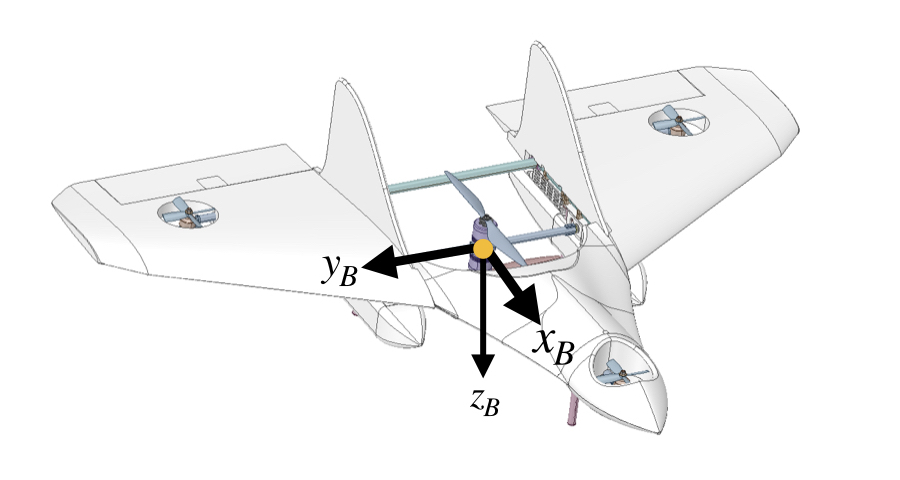
\includegraphics[clip,width=7.0cm,bb=0 0 900 480]{./z_figure_files/chapter3/1_body_axis.jpeg}
					\caption{Body coordinate frame}
					\label{fig:body_axis}
				\end{center}
			\end{minipage}
			\begin{minipage}{0.5\hsize}
				\begin{center}
					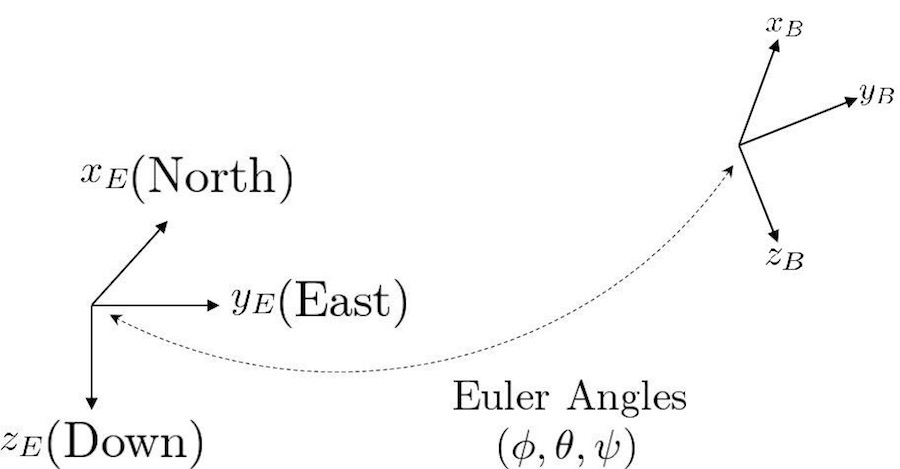
\includegraphics[clip,width=7.0cm,bb=0 0 900 480]{./z_figure_files/chapter3/2_NED.jpeg}
					\caption{NED coordinate system}
					\label{fig:ned_axis}
				\end{center}
			\end{minipage}
		\end{tabular}
	\end{center}
\end{figure}

\subsection{座標系の変換}

例えば,$a^{(E)}$から$a^{(B)}$への座標変換行列を$A^{(B,E)}$と書くとすると
\begin{equation}
  \left[
    \begin{array}{ccc}
      x \\
      y \\
      z
    \end{array}
  \right]_B =
  A^{(B,E)}
  \left[
    \begin{array}{ccc}
      x \\
      y \\
      z
    \end{array}
  \right]_E
\end{equation}
となり
\begin{equation}
  \begin{split}
    A^{(B,E)} &=
    \left[
      \begin{array}{ccc}
        1 & 0 & 0 \\
        0 & c\phi & s\phi \\
        0 & -s\phi & c\phi
      \end{array}
    \right]
    \left[
      \begin{array}{ccc}
        c\theta & 0 & -s\theta \\
        0 & 1 & 0 \\
        s\theta & 0 & c\theta
      \end{array}
    \right]
    \left[
      \begin{array}{ccc}
        c\psi & s\psi & 0 \\
        -s\psi & c\psi & 0 \\
        0 & 0 & 1
      \end{array}
    \right] \\
    &=
    \left[
  	\begin{array}{ccc}
    	c\theta c\psi & c\theta s\psi & -s\theta \\
    	s\phi s\theta c\psi - c\phi s\psi & s\phi s\theta s\psi + c\phi c\psi & s\phi c\theta \\
    	c\theta s\theta c\psi + s\phi s\psi & c\phi s\theta s\psi - s\phi c\psi & c\phi c\theta
  	\end{array}
  	\right]
  \end{split}
\end{equation}
のように表される.簡略のため,$\sin* = s*$,$\cos* = c*$と表記している.

また,$A^{(B,E)}$は直交行列であり,逆行列は転置行列に等しいため
\begin{equation}
  A^{(E,B)} =
  \left[
  \begin{array}{ccc}
    c\theta c\psi & s\phi s\theta c\psi - c\phi s\psi & c\theta s\theta c\psi + s\phi s\psi \\
    c\theta s\psi & s\phi s\theta s\psi + c\phi c\psi & c\phi s\theta s\psi - s\phi c\psi \\
    -s\theta & s\phi c\theta & c\phi c\theta
  \end{array}
  \right]
\end{equation}
となる.

\subsection{オイラー角の微分方程式}

オイラー角と機体角速度の関係は
\begin{equation}
  \left[
  \begin{array}{ccc}
    \dot{\phi} \\
    \dot{\theta} \\
    \dot{\psi}
  \end{array}
  \right]
   =
  \left[
  \begin{array}{ccc}
    1 & \sin\phi\tan\theta & \cos\phi\tan\theta \\
    0 & \cos\phi & -\sin\phi \\
    0 & \frac{\sin\phi}{\cos\theta} & \frac{\cos\phi}{\cos\theta}
  \end{array}
  \right]
  \left[
  \begin{array}{ccc}
    p \\
    q \\
    r
  \end{array}
  \right]
  \label{eq:euler}
\end{equation}
となる.ただし,
\begin{equation*}
  \mbox{\boldmath $\omega$} =
  \left[
  \begin{array}{c}
    p \quad q \quad r
  \end{array}
  \right]^{\mathrm{T}} :
  \mbox{機体の角速度}
\end{equation*}

これはオイラー角のキネマティクス方程式とよばれる\cite{shimada}.$\dot{\phi},\dot{\theta},\dot{\psi}$はそれぞれ姿勢角の時間微分である.

%%%%%%%%%%%%%%%%%%%%%%
\section{非線形モデル}
\label{sec:nonlin_model}
%%%%%%%%%%%%%%%%%%%%%%

並進運動と回転運動について,\cite{katayanagi}に倣ってそれぞれ運動方程式を記述する.その後,回転翼機モードでの低速飛行における縦運動の運動方程式についてまとめ,機体の非線形モデルとして設定する.

\subsection{非線形並進運動方程式}

機体座標系で表した並進運動方程式は,機体重量を$m$として
\begin{equation}
  \left[
  \begin{array}{ccc}
    \dot{u} \\
    \dot{v} \\
    \dot{w}
  \end{array}
  \right]
   =
  \left[
  \begin{array}{rrr}
    0 & r & -q \\
    -r & 0 & p \\
    q & -p & 0
  \end{array}
  \right]
  \left[
  \begin{array}{ccc}
    u \\
    v \\
    w
  \end{array}
  \right] + \dfrac{1}{m}
  \left[
  \begin{array}{ccc}
    F_x \\
    F_y \\
    F_z
  \end{array}
  \right]
  \label{eq:mot_eq}
\end{equation}
となる.ただし,
\begin{equation*}
  \mbox{\boldmath $V_g$} =
  \left[
  \begin{array}{c}
    u \quad v \quad w
  \end{array}
  \right]^{\mathrm{T}} :
  \mbox{機体の対地速度}
\end{equation*}
\begin{equation*}
  \mbox{\boldmath $F$} =
  \left[
  \begin{array}{c}
    F_x \quad F_y \quad F_z
  \end{array}
  \right]^{\mathrm{T}} :
  \mbox{機体に働く力}
\end{equation*}

式(\ref{eq:mot_eq})の右辺第2項の力は,重力,空気力,ロータ推力に分けて
\begin{equation}
    \mbox{\boldmath $F$} = \mbox{\boldmath $F_g$} + \mbox{\boldmath $F_a$} + \mbox{\boldmath $F_t$}
\end{equation}
\begin{align*}
  \mbox{\boldmath $F_g$} =
  \left[
  \begin{array}{c}
    X_g \quad Y_g \quad Z_g
  \end{array}
  \right]^{\mathrm{T}},
  \mbox{\boldmath $F_a$} =
  \left[
  \begin{array}{c}
    X_a \quad Y_a \quad Z_a
  \end{array}
  \right]^{\mathrm{T}},
  \mbox{\boldmath $F_t$} =
  \left[
  \begin{array}{c}
    X_t \quad Y_t \quad Z_t
  \end{array}
  \right]^{\mathrm{T}}
\end{align*}
と書ける.ここで重力について
\begin{equation}
  \mbox{\boldmath $F_g$} \triangleq
  \left[
  \begin{array}{ccc}
    X_g \\
    Y_g \\
    Z_g
  \end{array}
  \right] =
  A^{(B,E)}
  \left[
  \begin{array}{ccc}
    0 \\
    0 \\
    mg
  \end{array}
  \right] = mg
  \left[
  \begin{array}{ccc}
    -\sin\theta \\
    \sin\phi\cos\theta \\
    \cos\phi\cos\theta
  \end{array}
  \right]
  \label{eq:F_g}
\end{equation}
である.またロータ推力について,$y$軸方向の力$Y_t=0$であるから,ティルト角を$\gamma$,メインロータ推力を$T_m$,右左サブロータ推力を$T_r$,機首サブロータ推力を$T_f$とすれば次のようになる.
\begin{equation}
  \mbox{\boldmath $F_t$} \triangleq
  \left[
    \begin{array}{ccc}
      X_t \\
      Y_t \\
      Z_t
    \end{array}
  \right] =
  \left[
    \begin{array}{ccc}
      -\cos\gamma & 0 & \sin\gamma \\
      0 & 0 & 0 \\
      -\sin\gamma & 0 & -\cos\gamma
    \end{array}
  \right]
  \left[
    \begin{array}{ccc}
      0 \\
      0 \\
      T_m
    \end{array}
  \right] -
  \left[
    \begin{array}{ccc}
      0 \\
      0 \\
      T_r + T_f
    \end{array}
  \right]
  \label{eq:F_t}
\end{equation}

空気力項については,\ref{sec:airf_model}節で詳しく述べる.

% \begin{equation}
%   \left[
%   \begin{array}{ccc}
%     \dot{u} \\
%     \dot{v} \\
%     \dot{w}
%   \end{array}
%   \right]
%    =
%   \left[
%   \begin{array}{rrr}
%     0 & r & -q \\
%     -r & 0 & p \\
%     q & -p & 0
%   \end{array}
%   \right]
%   \left[
%   \begin{array}{ccc}
%     u \\
%     v \\
%     w
%   \end{array}
%   \right] + g
%   \left[
%   \begin{array}{ccc}
%     -\sin\theta \\
%     \sin\phi\cos\theta \\
%     \cos\phi\cos\theta
%   \end{array}
%   \right] + \dfrac{1}{m}
%   \left[
%   \begin{array}{ccc}
%     X_a + X_t \\
%     Y_a + Y_t \\
%     Z_a + Z_t
%   \end{array}
%   \right]
% \end{equation}

\subsection{非線形回転運動方程式}

次に,回転の運動について考える.本研究で開発した機体は,機体座標系における$x$軸と$z$軸で張られる面に対し面対称であるため,慣性乗積を0とすると,慣性行列は次のようになる.
\begin{equation}
  I =
  \left[
  \begin{array}{ccc}
    I_{xx} & 0 & -I_{xz} \\
    0 & I_{yy} & 0 \\
    -I_{xz} & 0 & I_{zz}
  \end{array}
  \right]
\end{equation}
このとき,機体の回転運動方程式は
\begin{equation}
I\left[
  \begin{array}{ccc}
    \dot{p} \\
    \dot{q} \\
    \dot{r}
  \end{array}
  \right] =
  \left[
  \begin{array}{rrr}
    0 & r & -q \\
    -r & 0 & p \\
    q & -p & 0
  \end{array}
  \right]
  I
  \left[
  \begin{array}{ccc}
    p \\
    q \\
    r
  \end{array}
  \right] +
  \left[
  \begin{array}{ccc}
    L \\
    M \\
    N
  \end{array}
  \right]
  \label{eq:roll_eq}
\end{equation}
となる.ただし,
\begin{equation*}
  \mbox{\boldmath $M$} =
  \left[
  \begin{array}{c}
    L \quad M \quad N
  \end{array}
  \right]^{\mathrm{T}} :
  \mbox{各機体軸まわりのモーメント}
\end{equation*}

式(\ref{eq:roll_eq})の右辺第2項のモーメントは,重力,空気力,ロータ推力それぞれによるモーメントに分けて
\begin{equation}
    \mbox{\boldmath $M$} = \mbox{\boldmath $M_g$} + \mbox{\boldmath $M_a$} + \mbox{\boldmath $M_t$}
\end{equation}
\begin{align*}
  \mbox{\boldmath $M_g$} =
  \left[
  \begin{array}{c}
    L_g \quad M_g \quad N_g
  \end{array}
  \right]^{\mathrm{T}},
  \mbox{\boldmath $M_a$} =
  \left[
  \begin{array}{c}
    L_a \quad M_a \quad N_a
  \end{array}
  \right]^{\mathrm{T}},
  \mbox{\boldmath $M_t$} =
  \left[
  \begin{array}{c}
    L_t \quad M_t \quad N_t
  \end{array}
  \right]^{\mathrm{T}}
\end{align*}
と書ける.ここで重力について,機体軸原点から重心までの距離ベクトルを\mbox{\boldmath $R_G$}とすれば,式(\ref{eq:F_g})も考慮して
\begin{equation}
  \begin{split}
    \mbox{\boldmath $M_g$} \triangleq
    \left[
    \begin{array}{ccc}
      L_g \\
      M_g \\
      N_g
    \end{array}
    \right] =
    \mbox{\boldmath $R_G$} \times
    m\mbox{\boldmath $g$} &=
    \left[
    \begin{array}{ccc}
      R_{G_x} \\
      0 \\
      R_{G_z}
    \end{array}
    \right] \times A^{(B,E)}
		  \left[
		  \begin{array}{ccc}
		    0 \\
		    0 \\
		    mg
		  \end{array}
    \right] \\
    &= mg
    \left[
    \begin{array}{ccc}
      -R_{G_z}\cos\theta\sin\phi \\
      -R_{G_z}\sin\theta - R_{G_x}\cos\theta\cos\phi \\
      R_{G_x}\cos\theta\sin\phi
    \end{array}
    \right]
  \end{split}
  \label{eq:M_g}
\end{equation}
である.また,ロータ推力によるモーメントは,\cite{yoshimura}によるとまだ未解明な点も多いため,本研究で扱う縦運動に関係するピッチングモーメント$M_t$のみ記載することにする.機体軸原点から各ロータまでの距離をFig. \ref{fig:distance}のように定めると
\begin{equation}
  M_t = -l_m T_m \cos\gamma + l_f T_f - l_{r_y} T_r
  \label{eq:M_t}
\end{equation}
となる.ただし,$l_m$は機体軸原点からメインロータまでの$x$軸方向の距離であり,本研究においては$l_m=0$である.空気力によるモーメントの項については,\ref{sec:airf_model}節で詳しく述べる.

\begin{figure}[H]
	\centering
	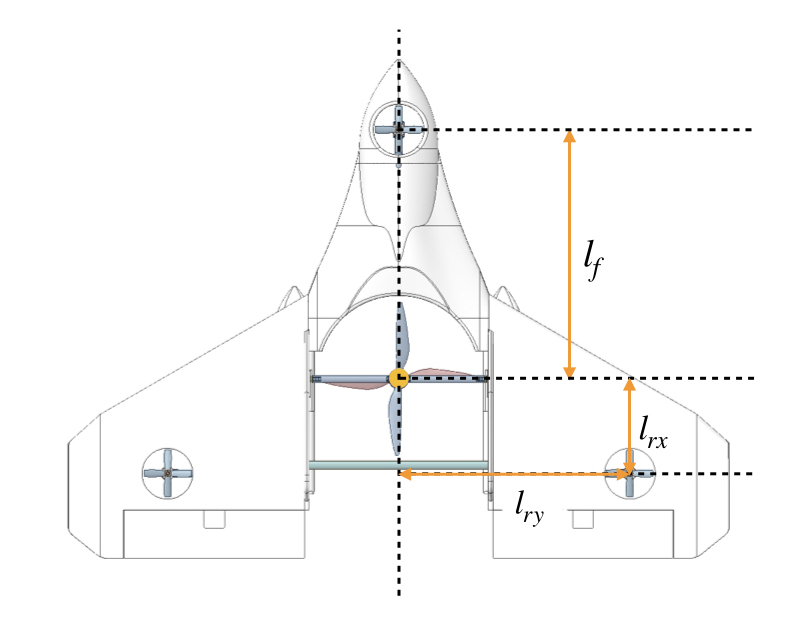
\includegraphics[clip,width=10.0cm,bb=0 0 800 630]{./z_figure_files/chapter3/3_distance.jpeg}
	\caption{Locations of rotors on the UAV}
	\label{fig:distance}
\end{figure}

\subsection{縦運動の非線形モデル}
\label{sec:lng_non_linear}

ここでは,Fig. \ref{fig:longtitude}に示すような縦運動を考える.そこで横・方向系の運動状態変数と入力変数を,$v=p=r=\delta_a=\phi=0$とすれば,縦運動における低速飛行の非線形モデルは式(\ref{eq:mot_eq}), 式(\ref{eq:F_g})および式(\ref{eq:roll_eq}), 式(\ref{eq:M_g})より,次のようになる.
\begin{align}
  \dot{u} &= -qw - g\sin\theta +\dfrac{1}{m}(X_a + X_t) \label{eq:u_dot} \\
  \dot{w} &= qu + g\cos\theta +\dfrac{1}{m}(Z_a + Z_t)  \\
  \dot{q} &= \dfrac{1}{I_{yy}}\left\{-mg(R_{G_z}\sin\theta+R_{G_x}\cos\theta\cos\phi) + M_a + M_t\right\} \label{eq:theta_dot}
\end{align}

加えて,式(\ref{eq:euler})より
\begin{equation}
  \dot{\theta} = q\cos\phi - r\sin\phi = q
\end{equation}
である.

\begin{figure}[H]
	\centering
	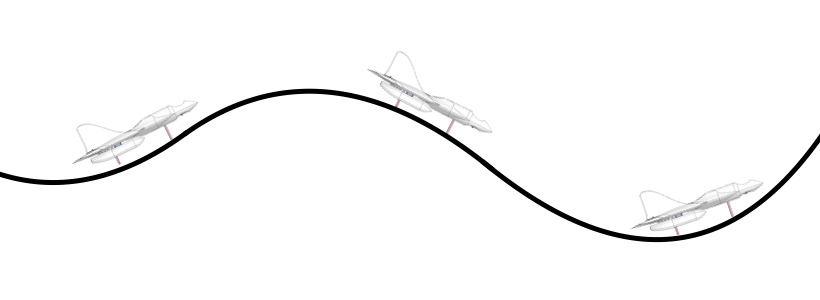
\includegraphics[clip,width=12.0cm,bb=0 0 820 300]{./z_figure_files/chapter3/4_longtitude.jpeg}
	\caption{Longtitudinal motion}
	\label{fig:longtitude}
\end{figure}


%%%%%%%%%%%%%%%%%%%%%%
\section{空気力モデル}
\label{sec:airf_model}
%%%%%%%%%%%%%%%%%%%%%%

本研究では,風が吹いている環境での回転翼機モードにおける低速飛行を想定する.そこで,まず機体の対気速度の設定を述べ,その後空気力モデルについてまとめ,\ref{sec:nonlin_model}節の空気力項について詳しく述べる.

\subsection{一定風下での対気速度}
\label{sec:wind_speed}

機体の対気速度$\mbox{\boldmath $V_a$}$,対地速度$\mbox{\boldmath $V_g$}$,風速$\mbox{\boldmath $V_w$}$の関係をFig. \ref{fig:vel_air}に示す.

\begin{figure}[H]
	\centering
	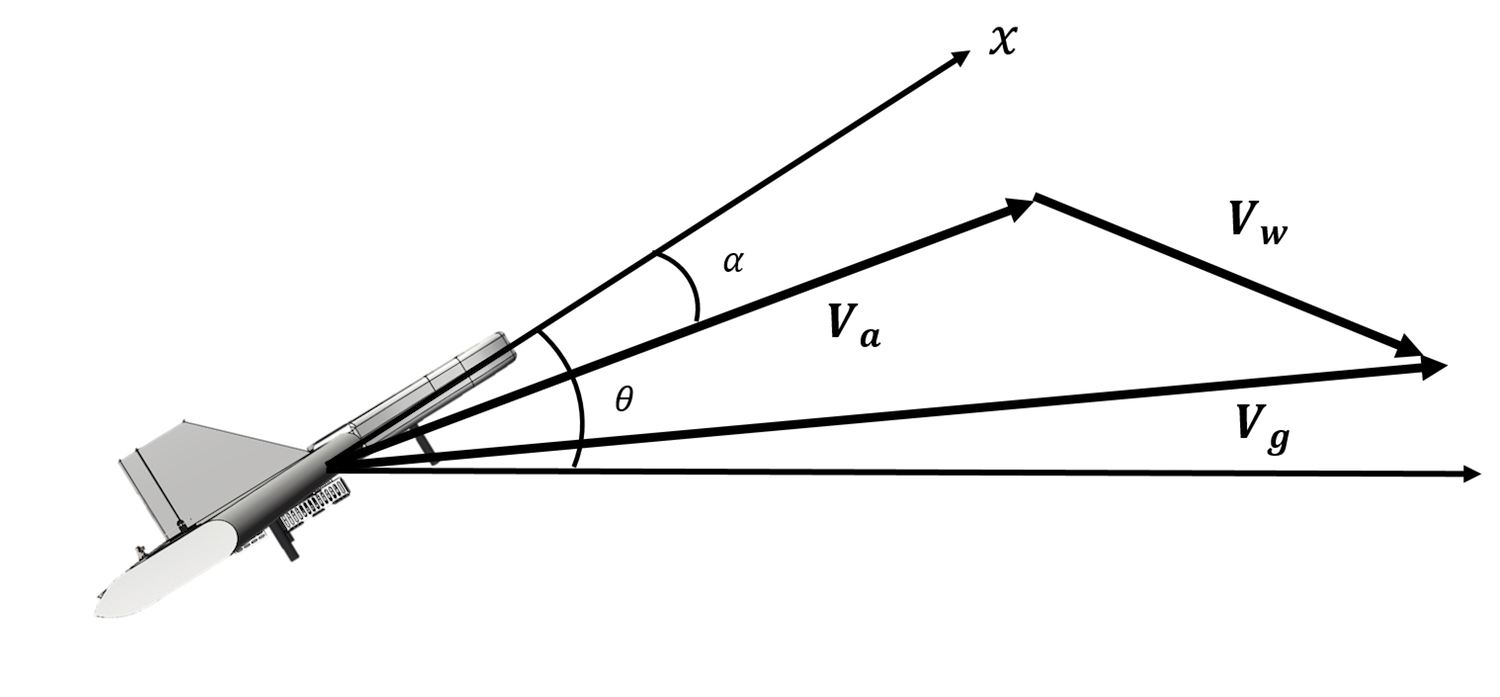
\includegraphics[clip,width=10.0cm,bb=0 0 1500 700]{./z_figure_files/chapter3/5_Va_Vw.jpeg}
	\caption{The wind triangle}
	\label{fig:vel_air}
\end{figure}

$\mbox{\boldmath $V_a$}$は,$\mbox{\boldmath $V_g$},\mbox{\boldmath $V_w$}$を用いて次のように表される.
\begin{equation}
  \mbox{\boldmath $V_a$} = \mbox{\boldmath $V_g$} - \mbox{\boldmath $V_w$}
\end{equation}
したがって,機体座標系における対気速度は
\begin{equation}
  \mbox{\boldmath $V_a$} \triangleq
  \left[
    \begin{array}{ccc}
      u_a \\
      v_a \\
      w_a
    \end{array}
  \right] =
  \left[
    \begin{array}{ccc}
      u \\
      v \\
      w \\
    \end{array}
  \right] -
  \left[
    \begin{array}{ccc}
      u_w \\
      v_w \\
      w_w
    \end{array}
  \right]
\end{equation}
となる.よって,対気速度\mbox{\boldmath $V_a$}の大きさを$V_a$とすると次のようになる.
\begin{equation}
  V_a = \sqrt{{u_a}^2+{v_a}^2+{w_a}^2}
\end{equation}
また,$\alpha$は迎角であり
\begin{equation}
  \alpha = \tan^{-1}\left(\dfrac{w_a}{u_a}\right)
\end{equation}
で計算される.

\subsection{対気速度により発生する空気力}
\label{sec:airspeed_airf}

ここで,Fig. \ref{fig:xz_force}の場合を想定する.まず,エレベータ舵角$\delta_e$とエルロン舵角$\delta_a$は,左右エレボン舵角$\delta_{e_l}, \delta_{e_r}$を用いて次のように表される.
\begin{equation}
  \left[
    \begin{array}{ccc}
      \delta_e \\
      \delta_a
    \end{array}
  \right] =
  \left[
    \begin{array}{ccc}
      1 & 1 \\
      -1 & 1
    \end{array}
  \right]
  \left[
    \begin{array}{ccc}
      \delta_{e_r} \\
      \delta_{e_l}
    \end{array}
  \right]
\end{equation}

対気速度$V_a$により発生する,速度と垂直方向に働く揚力$L$,水平方向に働く抗力$D$,およびピッチモーメント$M_a$は一般に
\begin{align}
  L &= \dfrac{1}{2}\rho V_a^2 S \underbrace{\left[ C_{L_0}
  +C_{L_\alpha}\alpha+C_{L_q}\dfrac{\bar{c}}{2V_a}q+C_{L_{\delta_e}}\delta_e \right]}_{C_L} \label{eq:L_o} \\
  D &= \dfrac{1}{2}\rho V_a^2 S \underbrace{\left[ C_{D_0}+\kappa {C_L}^2 \right]}_{C_D} \label{eq:D_o} \\
  M_a &= \dfrac{1}{2}\rho V_a^2 S \bar{c} \underbrace{\left[ C_{m_0}
  +C_{m_\alpha}\alpha+C_{m_q}\dfrac{\bar{c}}{2V_a}q+C_{m_{\delta_e}}\delta_e \right]}_{C_m} \label{eq:Ma_o}
\end{align}
と表される\cite{etkin}.ただし,$\rho$は大気密度,$S$は全機面積,$\bar{c}$は平均空力翼弦であり,$C_L,C_D$はそれぞれ揚力係数,抗力係数である.例えば$C_{L_\alpha}$は,迎角$\alpha$が増加したときにどれくらい$C_L$が増えるかを表したもので,このような空力係数は安定微係数とよばれる.

以上は一般的な空気力モデルであるが,ロータの吸い込みによって発生する,対気速度に比例する抗力\cite{yamana}と同様に対気速度に比例した揚力およびピッチモーメントが発生するとして,本研究ではモデル式を次のように変更している.
\begin{align}
  L &= \dfrac{1}{2}\rho {V_a}^2 S C_L + k_L V_a \label{eq:L} \\[5pt]
  D &= \dfrac{1}{2}\rho {V_a}^2 S C_D + k_D V_a \label{eq:D} \\[5pt]
  M_a &= \dfrac{1}{2}\rho {V_a}^2 S \bar{c} C_m + k_m V_a \label{eq:Ma}
\end{align}

また安定微係数について,一般の航空機では影響が小さいとして省略されていた項を考慮し
\begin{align}
  C_L &= C_{L_0}+C_{L_\alpha}\alpha+C_{L_{\dot{\alpha}}}\dfrac{\bar{c}}{2V_a}\dot{\alpha}+C_{L_q}\dfrac{\bar{c}}{2V_a}q+C_{L_{\delta_e}}\delta_e \label{eq:CL} \\[5pt]
  C_m &= C_{m_0}+C_{m_\alpha}\alpha+C_{m_{\dot{\alpha}}}\dfrac{\bar{c}}{2V_a}\dot{\alpha}+C_{m_q}\dfrac{\bar{c}}{2V_a}q+C_{m_{\delta_e}}\delta_e \label{eq:Cm}
\end{align}
とした.最後に,\ref{sec:nonlin_model}節の空気力項について
\begin{equation}
  \left[
  \begin{array}{ccc}
    X_a \\
    Z_a
  \end{array}
  \right] =
  \left[
  \begin{array}{ccc}
    \sin\alpha & -\cos\alpha \\
    -\cos\alpha & -\sin\alpha
  \end{array}
  \right]
  \left[
  \begin{array}{ccc}
    L \\
    D \\
  \end{array}
  \right]
  \label{eq:XZ_to_LD}
\end{equation}
と書ける.

$Y_a,L_a,N_a$についても同様な表現が可能だが,本研究では縦運動にのみ着目するためここでは述べない.

% $Y_a$は揚力や抗力と同様に
% \begin{equation}
%   Y_a = \dfrac{1}{2}\rho {V_a}^2 S C_Y + k_Y V_a
% \end{equation}
% と仮定する.

\begin{figure}[H]
	\centering
	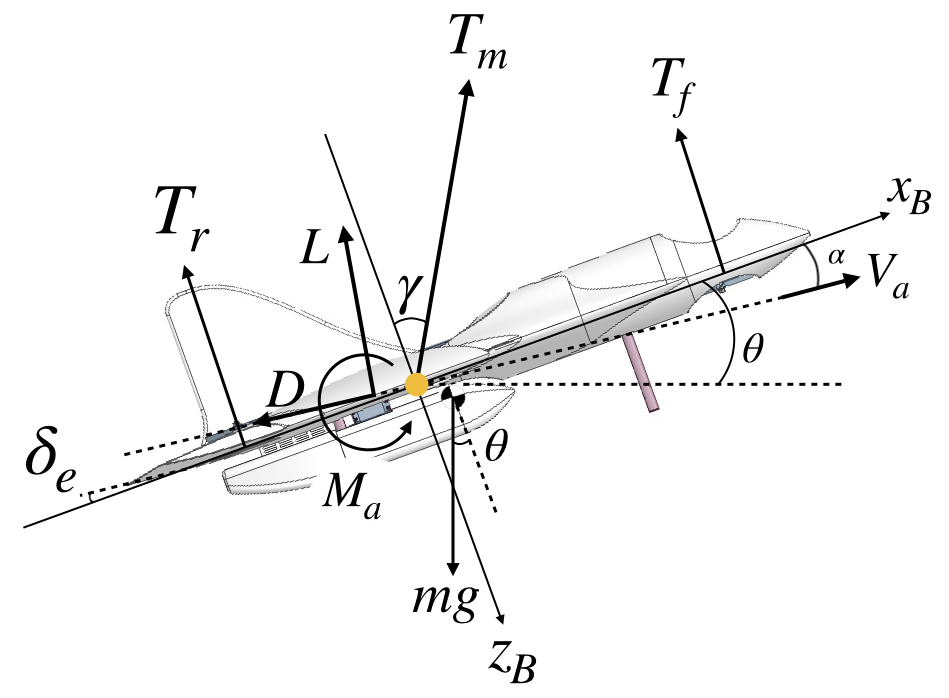
\includegraphics[clip,width=15.0cm,bb=0 0 935 551]{./z_figure_files/chapter3/6_xz_force.jpeg}
	\caption{Force and moment}
	\label{fig:xz_force}
\end{figure}

%%%%%%%%%%%%%%%%%%%%
\section{縦運動の線形モデル}
%%%%%%%%%%%%%%%%%%%%
本節では,縦運動を解析的に検討するために,\cite{katou}に倣って機体の運動を定常状態からの微小擾乱運動と仮定して近似を行なう.これにより,\ref{sec:nonlin_model}節の非線形モデルを線形化する.

\subsection{定常状態}
\label{sec:steady}

まず,回転翼機モードにおける定常状態の定義について述べる.定常状態での状態変数を,添字0を付けて表し,以下を仮定する.
	\begin{itemize}
	\item[(1)]機体加速度は$\dot{u_0} = 0$,$\dot{w_0} = 0$である.
	\item[(2)]角速度は$q_0 = 0$である.
  \item[(3)]$w_0$および$\alpha_0$は微小である.
  \item[(4)]$|u_0|$はある程度の大きさを持ち,$|w_0|\ll|u_0|$である.
	\end{itemize}

釣り合い条件として,運動方程式の加速度,モーメント,および外力の総和が0であるから
\begin{equation}
  \left\{
  \begin{align}
    X_{a0} &+ X_{t0} - mg\sin\theta_0 = 0 \\
    Z_{a0} &+ Z_{t0} + mg\cos\theta_0 = 0 \\
    M_{a0} &+ M_{t0} - mg(R_{G_z}\sin\theta_0 + R_{G_x}\cos\theta_0) = 0
  \end{align}
  \right
  \label{eq:balance}
\end{equation}

以下では,この定常状態からの微小変化を考える.また,定常状態が乱れたときの状態変数の変化を$\Delta$を付して書き
\begin{equation}
  \left\{
  \begin{align}
    u &= u_0 + \Delta u \\
    w &= w_0 + \Delta w \\
    V &= V_0 + \Delta V
  \end{align}
  \right
\end{equation}
\begin{equation}
  \left\{
  \begin{align}
    \alpha = \alpha_0 + \Delta \alpha = \tan^{-1}\left(\dfrac{w_0+\Delta w}{u_0+\Delta u}\right), \\
    \therefore \alpha_0 \fallingdotseq \tan^{-1}\left(\dfrac{w_0}{u_0}\right),\quad
    \Delta \alpha \fallingdotseq \dfrac{\Delta w}{u_0}
  \end{align}
  \right
  \label{eq:alpha_Delta}
\end{equation}
\begin{equation}
  \left\{
  \begin{align}
    q &\fallingdotseq \Delta q \\
    \theta &= \theta_0 + \Delta \theta,\quad \\
    &\therefore \sin\theta \fallingdotseq \sin\theta_0+\Delta\theta \cos\theta_0,\quad
    \cos\theta \fallingdotseq \cos\theta_0 - \Delta\theta \sin\theta_0
  \end{align}
  \right
\end{equation}
\begin{equation}
  \left\{
  \begin{align}
    X_a &= X_{a0} + \Delta X_a,\quad
    X_t = X_{t0} + \Delta X_t \\
    Z_a &= Z_{a0} + \Delta Z_a,\quad
    Z_t = Z_{t0} + \Delta Z_t \\
    M_a &= M_{a0} + \Delta M_a,\quad
    M_t = M_{t0} + \Delta M_t \\
  \end{align}
  \right
\end{equation}
\begin{equation}
  \delta_e = \delta_{e0} + \Delta \delta_e
\end{equation}
と近似する.これらを式(\ref{eq:u_dot})〜式(\ref{eq:theta_dot})に代入する.その後,式(\ref{eq:balance})を用いて変形し,速度と加速度の変化分が積で現れる項は微小であるとして無視すれば
\begin{align}
  \Delta \dot{u} &= -w_0 \Delta q - (g\cos\theta_0)\Delta \theta +\dfrac{1}{m}(\Delta X_a + \Delta X_t) \\
  \Delta \dot{w} &= u_0 \Delta q - (g\sin \theta_0)\Delta \theta +\dfrac{1}{m}(\Delta Z_a + \Delta Z_t) \\
  \Delta \dot{q} &= \dfrac{1}{I_{yy}}\left\{mg(R_{G_x}\sin\theta_0 - R_{G_z}\cos\theta_0)\Delta \theta + \Delta M_a + \Delta M_t\right\}
\end{align}
となる.

\subsection{空気力項の線形化}
\label{sec:airf_lin}

空気力項($X_a, Z_a, M_a$)のうちの1つを$A$で代表して表す.ティルト角$\gamma$は一定であるという条件下で,$A$は一般に機体の速度,角速度,舵角,およびロータ推力の関数であると仮定できる.いまそれらの釣り合い位置からの変化分を,$\Delta u,\Delta w,\Delta q,\Delta \delta_e$とし,これらはいずれも微小量とする.このとき,$A$を上記4変数についてテイラー級数に展開し,それぞれの第1項のみ用いると
\begin{equation}
    A \fallingdotseq A_0 &+ \dfrac{\partial A}{\partial \Delta u}\Delta u
    + \dfrac{\partial A}{\partial \Delta w}\Delta w
    + \dfrac{\partial A}{\partial \Delta q}\Delta q
    + \dfrac{\partial A}{\partial \Delta \delta e}\Delta \delta e
\end{equation}
と近似できる.ここで$A_0$は釣り合い時の値で,力に関しては$X_{a0},Z_{a0}$,モーメントに関しては$M_{a0}$である.また右辺に現れる微係数は,すべて釣り合い状態で定義される.このようにして求められる$A$の偏微分項は,一般に安定微係数とよばれる.

また,$Z_a,M_a$については,さらに$\dfrac{\partial Z_a}{\partial \Delta \dot{w}}\Delta \dot{w},\dfrac{\partial M_a}{\partial \Delta \dot{w}}\Delta \dot{w}$あるいは$\dfrac{\partial Z_a}{\partial \Delta \dot{\alpha}}\Delta \dot{\alpha},\dfrac{\partial M_a}{\partial \Delta \dot{\alpha}}\Delta \dot{\alpha}$の項を含める.

以上より,機体に作用する力とモーメントは次のように線形化される.
\begin{align}
  \Delta X_a &= \dfrac{\partial X_a}{\partial \Delta u}\Delta u
  + \dfrac{\partial X_a}{\partial \Delta w}\Delta w
  + \dfrac{\partial X_a}{\partial \Delta q}\Delta q
  + \dfrac{\partial X_a}{\partial \Delta \delta_e}\Delta \delta_e  \\
  \Delta Z_a &= \dfrac{\partial Z_a}{\partial \Delta u}\Delta u
  + \dfrac{\partial Z_a}{\partial \Delta w}\Delta w
  + \dfrac{\partial Z_a}{\partial \Delta \dot{w}}\Delta \dot{w}
  + \dfrac{\partial Z_a}{\partial \Delta q}\Delta q
  + \dfrac{\partial Z_a}{\partial \Delta \delta_e}\Delta \delta_e \\
  \Delta M_a &= \dfrac{\partial M_a}{\partial \Delta u}\Delta u
  + \dfrac{\partial M_a}{\partial \Delta w}\Delta w
  + \dfrac{\partial M_a}{\partial \Delta \dot{w}}\Delta \dot{w}
  + \dfrac{\partial M_a}{\partial \Delta q}\Delta q
  + \dfrac{\partial M_a}{\partial \Delta \delta_e}\Delta \delta_e
\end{align}

さらに式(\ref{eq:alpha_Delta})より
\begin{equation}
  \left\{
  \begin{align}
    \Delta \dot{w} &= u_0 \Delta \dot{\alpha} \\
    \dfrac{\partial A}{\partial \Delta w} &= \dfrac{1}{u_0}\left(\dfrac{\partial A}{\partial \Delta \alpha}\right) \\
    \dfrac{\partial A}{\partial \Delta \dot{w}} &= \dfrac{1}{u_0}\left(\dfrac{\partial A}{\partial \Delta \dot{\alpha}}\right)
  \end{align}
\end{equation}
であるから,まとめて
\begin{equation}
  \left\{
  \begin{align}
    \dfrac{\partial A}{\partial \Delta w}\Delta w &= \dfrac{\partial A}{\partial \Delta \alpha}\Delta\alpha \\
    \dfrac{\partial A}{\partial \Delta \dot{w}}\Delta \dot{w} &= \dfrac{\partial A}{\partial \Delta \dot{\alpha}}\Delta\dot{\alpha}
  \end{align}
  \label{eq:w_to_alpha}
\end{equation}

\subsection{線形化された縦運動モデル}
\label{sec:linear}

\ref{sec:steady}小節と\ref{sec:airf_lin}小節の内容をふまえ,式(\ref{eq:F_t})と式(\ref{eq:M_t})も考慮して,線形化した縦の運動方程式をまとめると次のようになる.ただし,式(\ref{eq:w_to_alpha})を用いて,$w$に関する式を$\alpha$に関する式に変換した上で,各項の係数を略記し
\begin{equation}
  \left\{
  \begin{align}
    \Delta \dot{u} &= X_u \Delta u + X_\alpha \Delta \alpha + X_q \Delta q + X_\theta \Delta \theta + X_{\delta_e} \Delta \delta_e + X_{T_m}\Delta T_m \\[3pt]
    \Delta \dot{\alpha} &= \overline{Z_u} \Delta u + \overline{Z_\alpha} \Delta \alpha + \overline{Z_q} \Delta q + \overline{Z_\theta} \Delta \theta \\
    &\qquad+ \overline{Z_{\delta_e}} \Delta \delta_e + \overline{Z_{T_m}}\Delta T_m + \overline{Z_{T_r}}\Delta T_r + \overline{Z_{T_f}}\Delta T_f \\[3pt]
    \Delta \dot{q} &= M_u \Delta u + M_\alpha \Delta \alpha + M_{\dot{\alpha}} \Delta \dot{\alpha} + M_q \Delta q + M_\theta \Delta \theta \\
    &\qquad+ M_{\delta_e} \Delta \delta_e + M_{T_m}\Delta T_m + M_{T_r} \Delta T_r + M_{T_f}\Delta T_f \\[3pt]
    \Delta \dot{\theta} &= \Delta q
  \end{align}
  \label{eq:lin_model_1}
\end{equation}
のように書ける.さらに式(\ref{eq:lin_model_1})において,$\Delta \dot{\alpha}$を用いて$\Delta \dot{q}$内の$\dot{\alpha}$を消去し,改めて線形化した縦運動モデルをまとめると
\begin{equation}
  \left\{
  \begin{align}
    \Delta \dot{u} &= X_u \Delta u + X_\alpha \Delta \alpha + X_q \Delta q + X_\theta \Delta \theta + X_{\delta_e} \Delta \delta_e + X_{T_m}\Delta T_m \\[3pt]
    \Delta \dot{\alpha} &= \overline{Z_u} \Delta u + \overline{Z_\alpha} \Delta \alpha + \overline{Z_q} \Delta q + \overline{Z_\theta} \Delta \theta \\
    &\qquad+ \overline{Z_{\delta_e}} \Delta \delta_e + \overline{Z_{T_m}}\Delta T_m + \overline{Z_{T_r}}\Delta T_r + \overline{Z_{T_f}}\Delta T_f \\[3pt]
    \Delta \dot{q} &= \overline{M_u} \Delta u + \overline{M_\alpha} \Delta \alpha + \overline{M_q} \Delta q + \overline{M_\theta} \Delta \theta \\
    &\qquad+ \overline{M_{\delta_e}} \Delta \delta_e + \overline{M_{T_m}}\Delta T_m + \overline{M_{T_r}} \Delta T_r + \overline{M_{T_f}}\Delta T_f \\[3pt]
    \Delta \dot{\theta} &= \Delta q
  \end{align}
  \label{eq:lin_model}
\end{equation}
のようになる.ただし
\begin{equation}
	\left\{
	\begin{align}
		X_u &= \frac{1}{m} \frac{\partial X_a}{\partial u},\quad
		X_\alpha = \frac{1}{m} \frac{\partial X_a}{\partial \alpha},\quad
		X_q = \frac{1}{m} \frac{\partial X_a}{\partial q} - w_0 \\[3pt]
		X_\theta &= -g\cos\theta_0,\quad
		X_{\delta_e} = \frac{1}{m} \frac{\partial X_a}{\partial \delta_e},\quad
		X_{T_m} = \frac{\sin\gamma}{m} \\[3pt]
		Z_u &= \frac{1}{m} \frac{\partial Z_a}{\partial u},\quad
		Z_\alpha = \frac{1}{m} \frac{\partial Z_a}{\partial \alpha},\quad
		Z_{\dot{\alpha}} = u_0 - \frac{1}{m} \frac{\partial Z_a}{\partial \dot\alpha} \\[3pt]
		Z_q &= \frac{1}{m} \frac{\partial Z_a}{\partial q} + u_0,\quad
		Z_\theta = -g\sin\theta_0,\quad
		Z_{\delta_e} = \frac{1}{m} \frac{\partial Z_a}{\partial \delta_e} \\[3pt]
		Z_{T_m} &= -\frac{\cos\gamma}{m},\quad
		Z_{T_r} = -\frac{1}{m},\quad
		Z_{T_f} = -\frac{1}{m} \\[3pt]
		M_u &= \frac{1}{I_{yy}} \frac{\partial M_a}{\partial u},\quad
		M_\alpha = \frac{1}{I_{yy}} \frac{\partial M_a}{\partial \alpha},\quad
		M_{\dot\alpha} = \frac{1}{I_{yy}} \frac{\partial M_a}{\partial \dot\alpha},\quad
		M_q = \frac{1}{I_{yy}} \frac{\partial M_a}{\partial q} \\[3pt]
		M_\theta &= \frac{mg}{I_{yy}}(R_{G_x}\sin\theta_0 - R_{G_z}\cos\theta_0),\quad
		M_{\delta_e} = \frac{1}{I_{yy}} \frac{\partial M_a}{\partial {\delta_e}} \\[3pt]
		M_{T_m} &= -\frac{l_m\cos\gamma}{I_{yy}},\quad
		M_{T_r} = -\frac{l_{r_x}}{I_{yy}},\quad
		M_{T_f} = \frac{l_f}{I_{yy}} \\[3pt]
		\overline{Z_*} &= \frac{Z_*}{Z_{\dot\alpha}},\quad
		\overline{M_*} = M_* + M_{\dot\alpha}\overline{Z_*}
	\end{align}
	\label{eq:partial_derivatives}
\end{equation}
